\chapter{Baseband VGA}%
\label{cha:Baseband VGA}

\section{Introduction}%
\label{sec:Introduction}
Baseband VGA main function is to give the ADC the required input
power in order to get the required SNR and not to saturate the 
ADC, the baseband VGA in this system is digitally controlled 
with 1dB step and control range of 15dB , here is the specification
table~\ref{tab:VGA_specs} 
\begin{table}[htpb]
    \centering
    \caption{Baseband VGA specifications}
    \label{tab:VGA_specs}


    \begin{tabular}{|c|c|}
        \hline
        \textbf{Parameter} & \textbf{Value} \\ \hline
        Maximum Gain  & 39dB  \\ \hline
        NF at maximum gain & 3dB \\ \hline
        OIP3 & 25dBm \\ \hline
        Control range & 15 dB (1dB step) \\ \hline
        BW & $\geq$ 600 MHz \\ \hline
    \end{tabular}
\end{table}

\section{Literature Review}%
\label{sec:Literature Review}
\subsection{Performance Metrics}%
\label{sub:Performance Metrics}
Here are key performance metrics are discussed and how it affects
the overall system lineup
\subsubsection{Max gain}%
Maximum gain affects the sensitivity of the receiver , VGA should
output sufficient voltage swing to ADC.
\subsubsection{Control Range}%
\label{ssub:Control Range}
Control Range affects the maximum input power the system can handle
,large control range means large input power range.
\subsubsection{Gain Error}%
\label{ssub:Gain Error}
Gain Error has two important metrics one is the DNL (Differential
Non-linearity) and the other is INL (Internal Non-linearity),
the first describe how much the step varies from ideal required
step (in our case 1dB) and the latter is how much the step varies
from its ideal value, DNL and INL equation are shown below.
\begin{equation}
    DNL = \frac{G(i+1)-G(i)}{\Delta G_{req.}}
    \label{eq:VGA_DNL}
\end{equation}
\begin{equation}
    INL = \sum_0^{i-1}{DNL(k)}
    \label{eq:VGA_INL}
\end{equation}
Where G(i) is the current gain state and $\Delta G_{req}$ is the
required step
\subsubsection{Input referred noise}%
\label{ssub:Input referred noise}
Noise requirements for VGA usually not very important but since
the chain before it is very lossy noise due to VGA should be 
sufficiently low.

\subsubsection{Linearity}%
Non-linear distortion caused by inter-modulation products and 
compression is very critical in our system  since VGA delivers
high voltage swing (after ADC input full-scale modification),
required OIP3 = 25 dBm 

\subsection{Types of VGAs}%
\subsubsection{Amp-Att Vs Att-Amp}%
\label{ssub:Amp-Att Vs Att-Amp}
VGAs can fall into two main categories one is Amplifier-Attenuator
and the other is Attenuator-Amplifier.\\
Amplifier-Attenuator provide constant noise figure across the 
states and constant IIP3 while OIP3 decreases dB-by-dB.\\
On the other hand Attenuator-Amplifier provide constant OIP3
with the states , IIP3 increase dB-by-dB  and Noise figure 
decreases dB-by-dB.
\begin{figure}[htpb]
    \centering
    
\includegraphics[width=0.8\textwidth]{VGA_fig.eps}
    \caption{Amp.-Att. Vs Att.-Amp.}
    \label{fig:amp_att_att_amp}
\end{figure}
\subsubsection{Open loop topologies}%
\label{ssub:Open loop topologies}
Open loop gain control usually gives good noise performance 
(No feedback resistance) but usually has poor linearity , here
are two open-loop topologies \cite{VGA_survey}, first 
is a basic bias current control (Figure~\ref{fig:VGA_basic_bias_control.png}), this topology suffers from very limited control range
gain $\propto \sqrt{I_{SS}}$ , the other topology has the same 
limitation but can get double the control range of the first 
topology,

\begin{figure}[htbp]
  \centering
  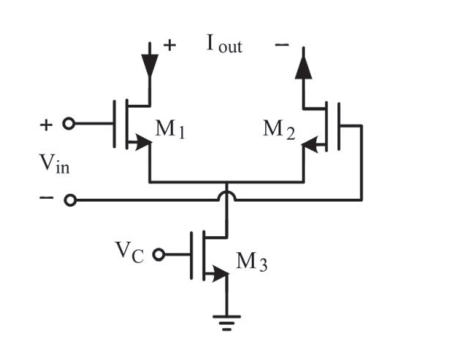
\includegraphics[width=0.4\linewidth]{images/VGA_basic_bias_control.png}
  \caption{VGA basic bias control \cite{VGA_survey}}
  \label{fig:VGA_basic_bias_control.png}
\end{figure}

\begin{figure}[htbp]
  \centering
  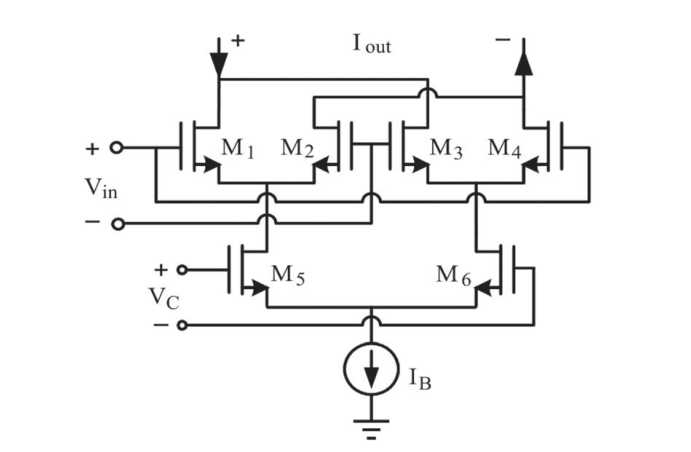
\includegraphics[width=0.6\linewidth]{images/VGA_gilbert_cell.png}
  \caption{Analog multiplier VGA \cite{VGA_survey} }
  \label{fig:VGA_gilbert_cell.png}
\end{figure}

\subsubsection{Feedback- topologies}%
\label{ssub:Feedback- topologies}
Topologies depends on feedback gives good linearity,here are 
couple of them:\\
first is the degeneration control 
(Figure~\ref{fig:VGA_resistive_degeneration.png}), this topology
has trade-off between linearity , noise  and power consumption,
although the linearity of this topology not very high compared
to closed loop topologies.\\
other resistive closed loop amplifiers gives better linearity 
performance but poor NF ( Figure~\ref{fig:VGA_closed_loop.png})

\begin{figure}[htbp]
  \centering
  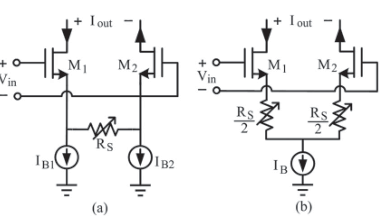
\includegraphics[width=0.8\linewidth]{images/VGA_resistive_degeneration.png}
  \caption{VGA  degeneration Control \cite{VGA_survey}}
  \label{fig:VGA_resistive_degeneration.png}
\end{figure}

\begin{figure}[htbp]
  \centering
  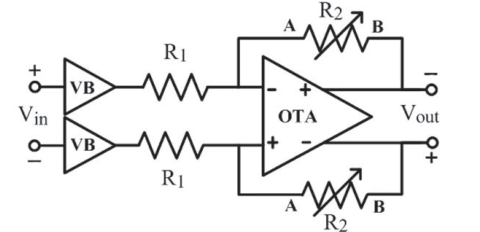
\includegraphics[width=0.8\linewidth]{images/VGA_closed_loop.png}
  \caption{Resistive feedback VGA}
  \label{fig:VGA_closed_loop.png}
\end{figure}

\section{Design Procedure}%
\label{sec:Design Procedure}
Given the requirements of both low NF and high linearity , there
is no single stage that can do both specially for high gain 
39dB , so VGA is divided into two parts: one which is LNA and 
the other is a resistive feedback Opamp which has good linearity 
but low noise figure.

It's required for the LNA stage to have noise figure of 2dB , 
Gain of 20dB and OIP3 = 15dBm, Gain variability will be chosen
to maximize total OIP3 , this is achieved later by varying the LNA 
stage by 10 dB and the rest 5 dB for the resistive feedback OPamp

For the resistive feedback Opamp stage OIP3 $\geq 27dBm$ , 
Gain of 19dB  and NF $\leq$ 15dB.
This gives us total NF of 2.7dB and OIP3 of 26.2dB at maximum
gain.

\subsubsection{LNA stage}%
\label{ssub:LNA stage}
To get a very low noise figure open-loop architecture has to 
be used but this gives low linearity , architecture in 
Figure~\ref{fig:LNA_literature_architecture.png} is used as the 
base for the LNA architecture but achieving gain = 10 dB with 
good linearity is hard for this architecture, so adding another
current mirror stage to get amplification almost has no effect 
on linearity , this can achieves the required 15dBm OIP3.

\begin{figure}[htbp]
  \centering
  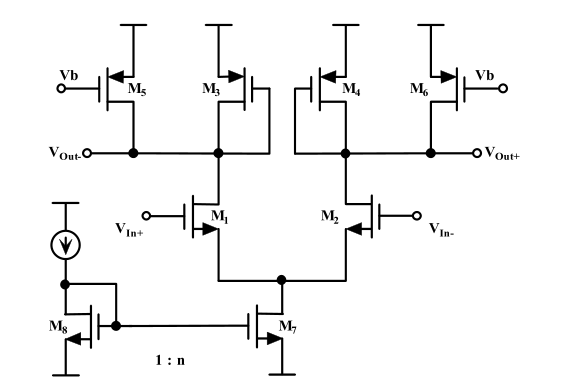
\includegraphics[width=0.8\linewidth]{images/LNA_literature_architecture.png}
  \caption{LNA basic architecture \cite{low_distorion_current_feedback} }
  \label{fig:LNA_literature_architecture.png}
\end{figure}

Another Modification is needed which to drive a low impedance 
resistive feedback Amplifier , so the output stage of the LNA
better to be low impedance.\\
Lastly, adding gain variability  to the LNA , current feedback 
is chosen \cite{low_distorion_current_feedback} because
degeneration resistive would be difficult
(very low resistive degeneration ) and load current control could
lead to huge power consumption across states.\\
Final LNA architecture is shown in Figure~\ref{fig:images-VGA_LNA_stage-eps}
\begin{figure}[htpb]
    \centering
    
\includegraphics[width=0.8\textwidth]{VGA_LNA_stage.eps}
    \caption{VGA LNA stage final architecture}
    \label{fig:images-VGA_LNA_stage-eps}
\end{figure}

\subsubsection{Resistive feedback Opamp}%
\label{ssub:Resisitive feedback Opamp}
For this stage that has very high linearity, it should be 
a resistive feedback with wide swing Opamp \cite{resistive_feedback_VGA},
architecture is shown in Figure~\ref{fig:vga_second_stage} and Figure~\ref{fig:VGA_Opamp_miller-eps}.\\
Although miller feedback limits BW and not suitable for high 
frequencies , in this architecture second stage is used as a
buffer instead of a Source follower stage which is a not a very
good buffer.\\
Also miller capacitance is changed with the state since the loop
gain is changing maintaining constant BW across state with 
good PM across all states.

\begin{figure}[htpb]
    \centering
    
\includegraphics[width=0.8\textwidth]{VGA_second_stage.eps}
    \caption{VGA second stage : resistive feedback stage}
    \label{fig:vga_second_stage}
\end{figure}
\begin{figure}[htpb]
    \centering
    
\includegraphics[width=0.8\textwidth]{VGA_Opamp_miller.eps}
    \caption{VGA second stage Opamp : miller compensated}
    \label{fig:VGA_Opamp_miller-eps}
\end{figure}

\subsubsection{Resistive and Capacitive DACs}%
\label{ssub:Resisitive and Capacitive DACs}
Resistive and Capacitive DACs switches are thin oxide mos switches
to reduce parasitics , but since OP voltage levels are different
we cannot use VDD and 0 to drive these switches, for 
miller compensation Capacitive DACs , Common mode voltage 
is around 0.5V , we cannot use VDD to the NMOS thin gate oxide
so instead we drive it with 1.2V , for the LNA resistive feedback
we used PMOS instead since VOCM is greater than 0.8V with VON = 0.4
and VOFF = 1.6 and for the resistive feedback for second stage 
VON =1.6V and VOFF=0V with nmos switches (Figure~\ref{fig:VGA_DAC-eps})
\begin{figure}[htpb]
    \centering
    
\includegraphics[width=0.8\textwidth]{VGA_DAC.eps}
    \caption{VGA DACs variability}
    \label{fig:VGA_DAC-eps}
\end{figure}

\section{Simulation Results}%
\label{sec:Simulation Results}
\subsection{AC Results}%
\label{sub:AC Results}
Simulation of full VGA is presented , input referred noise
at max gain = 24$\mu V$ which is equivalent to 2.7 dB, results
Figure~\ref{fig:DNL_across_states.png} shows a very small DNL
$\leq 0.1dB$ which is expected from schematic results, BW appears
to be constant around 625MHz Figure~\ref{fig:BW_across_state.png},
also minimum phase margin  is 64 deg. , AC results summary is 
shown in Table~\ref{tab:VGA_AC_results}

\begin{figure}[htbp]
  \centering
  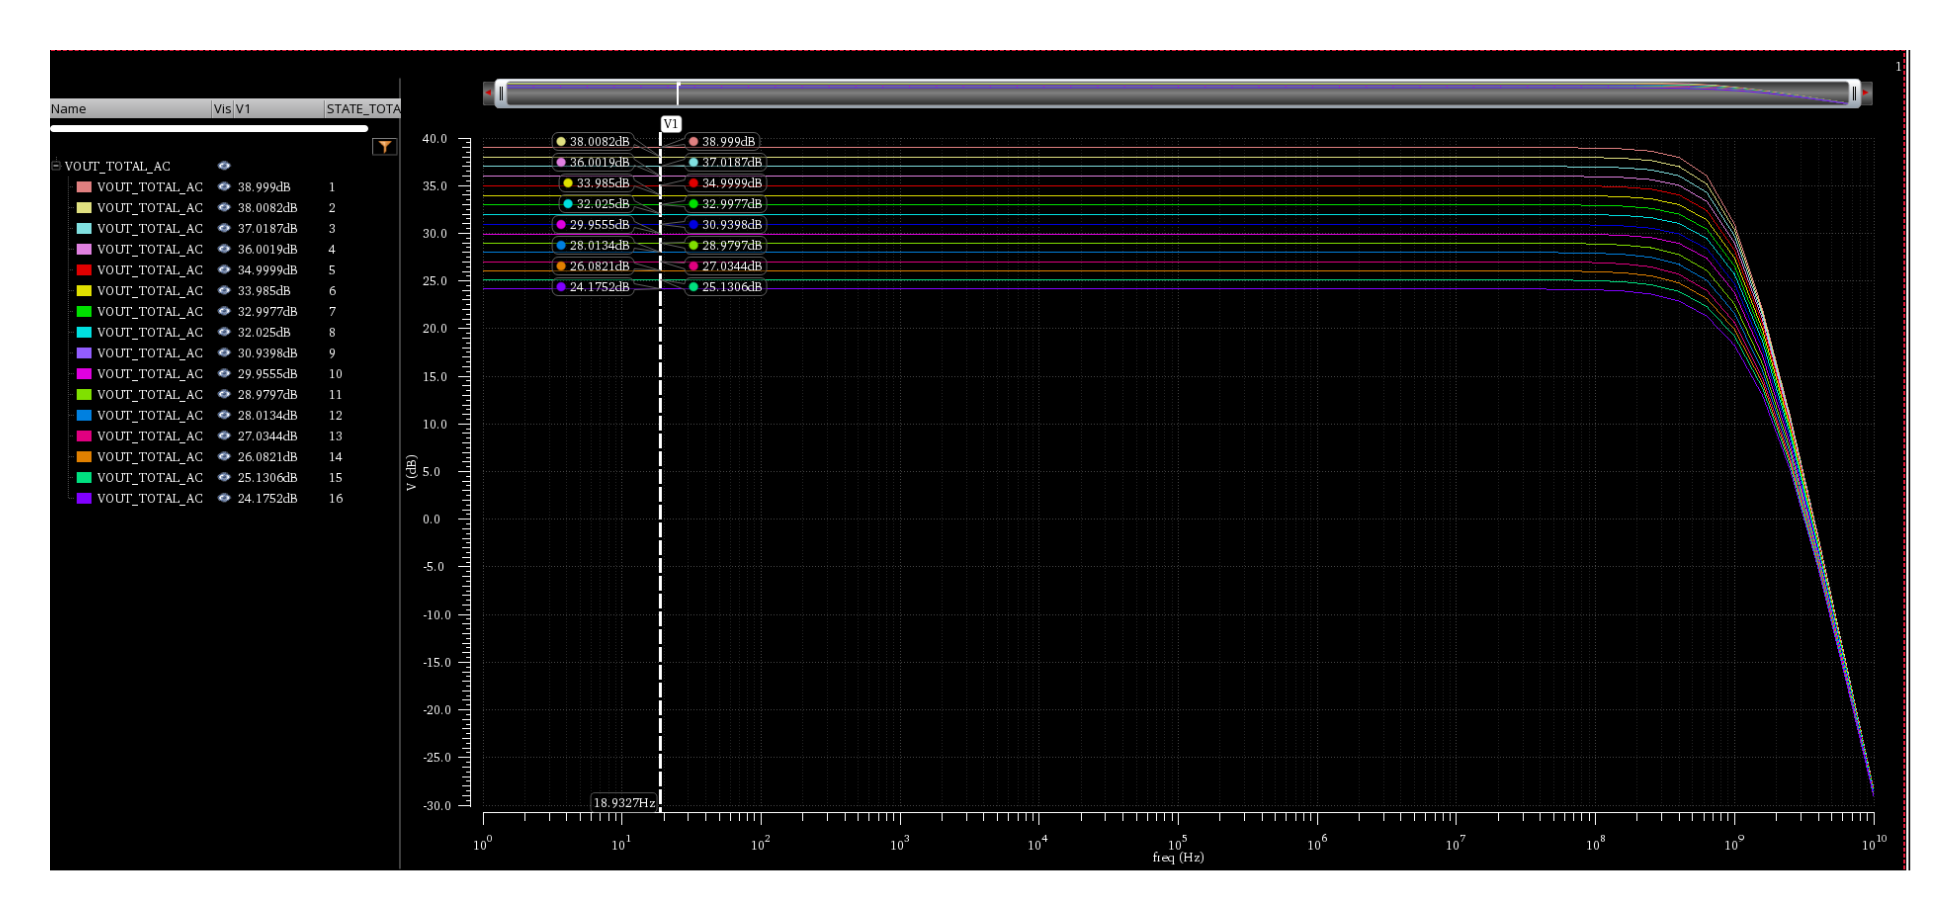
\includegraphics[width=1\linewidth]{images/AC_magnitude_plot_Vs_state.png}
  \caption{Small signal gain vs frequency across states}
  \label{fig:AC_magnitude_plot_Vs_state.png}
\end{figure}

\begin{figure}[htbp]
  \centering
  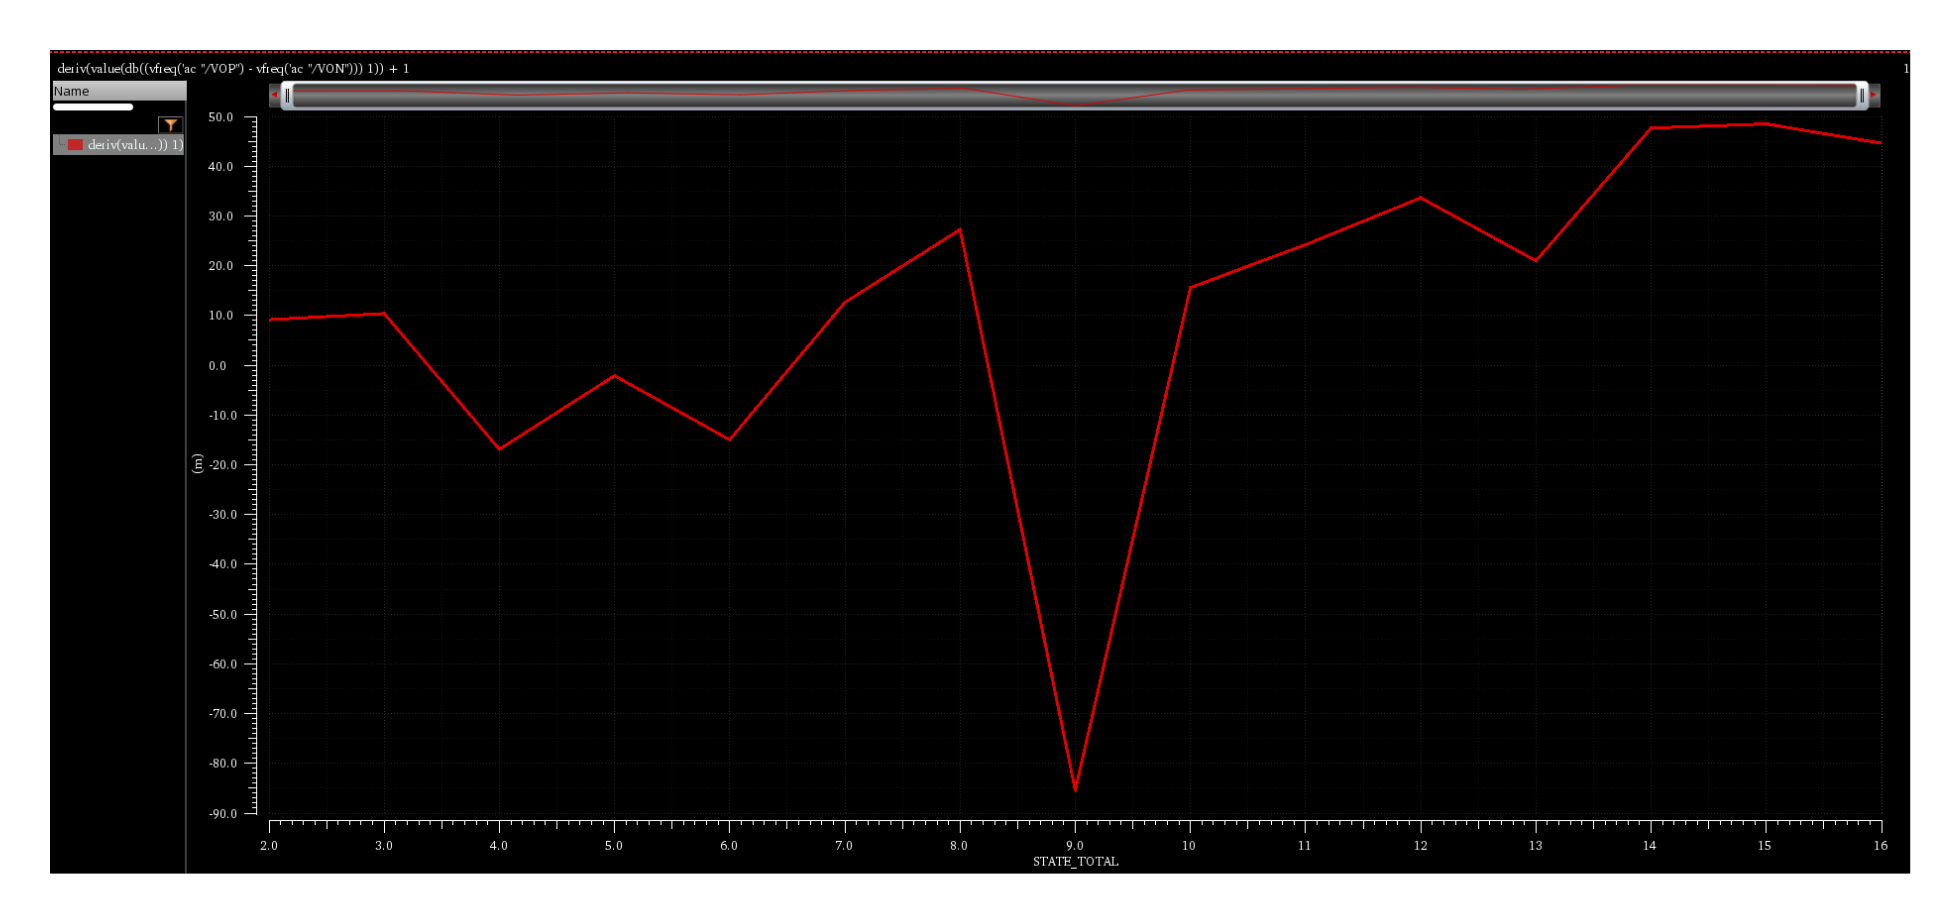
\includegraphics[width=1\linewidth]{images/DNL_across_states.png}
  \caption{DNL across states}
  \label{fig:DNL_across_states.png}
\end{figure}

\begin{figure}[htbp]
  \centering
  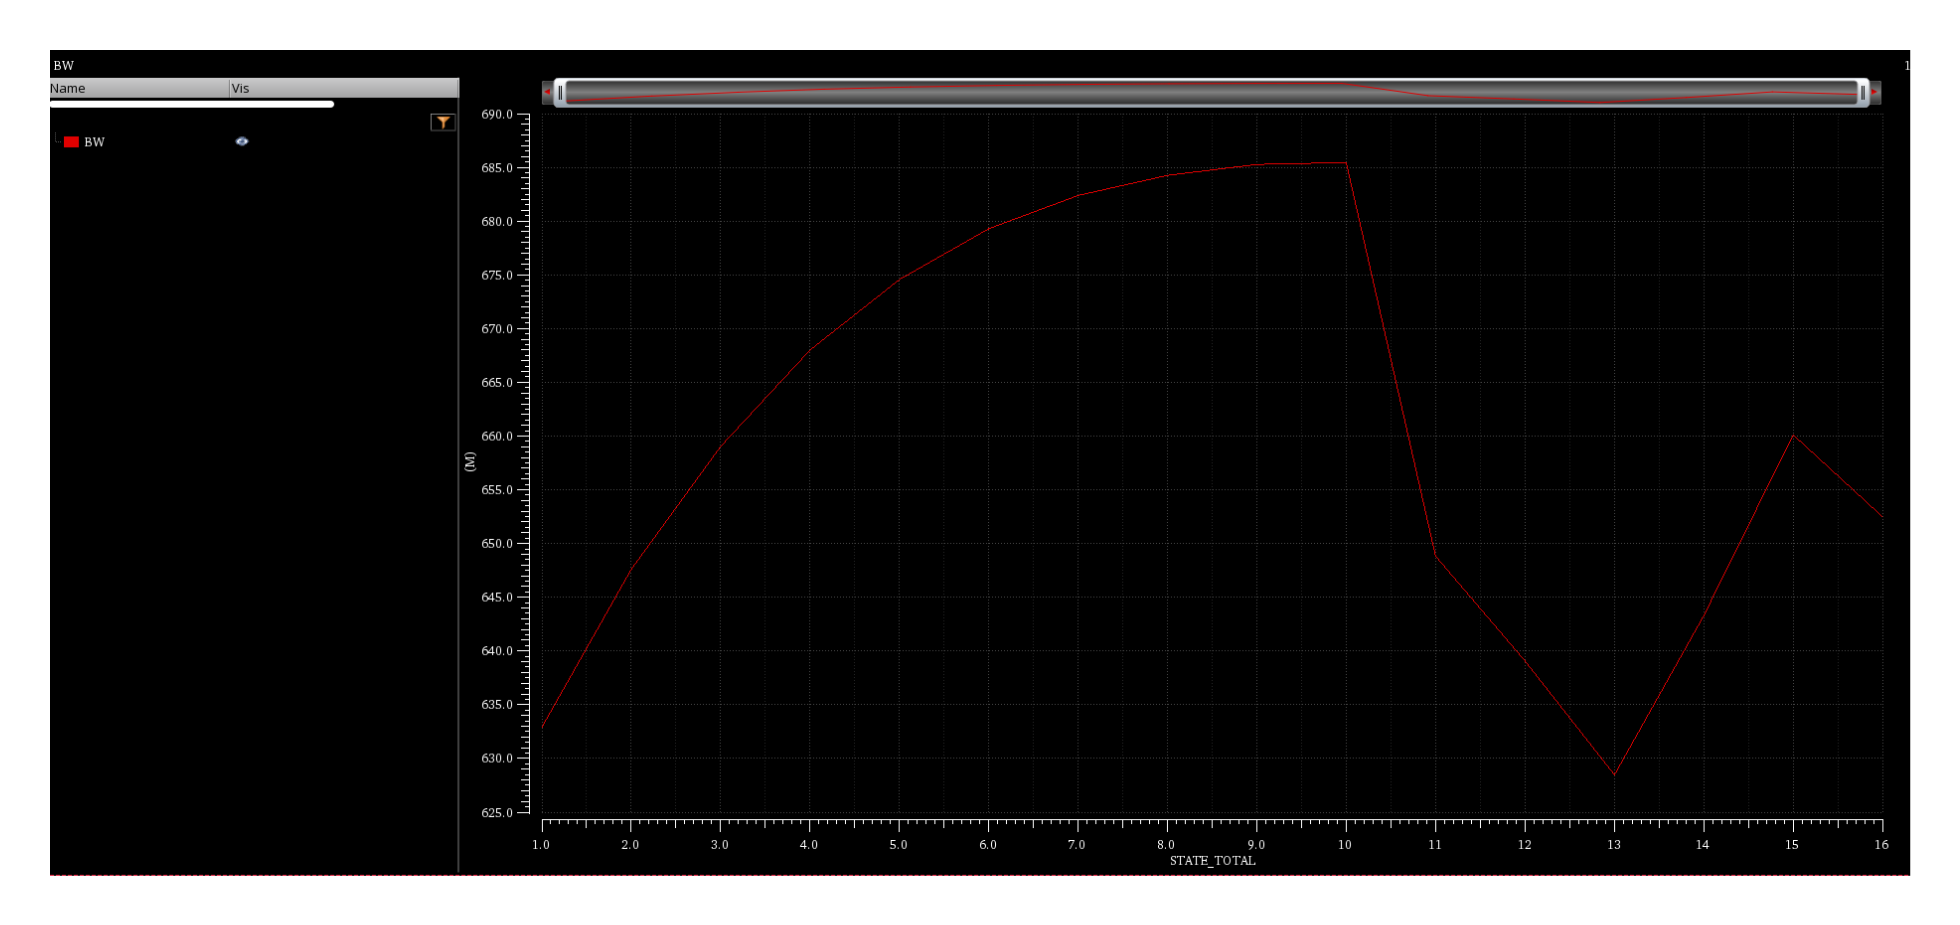
\includegraphics[width=1\linewidth]{images/BW_across_state.png}
  \caption{BW across states}
  \label{fig:BW_across_state.png}
\end{figure}

\begin{figure}[htbp]
  \centering
  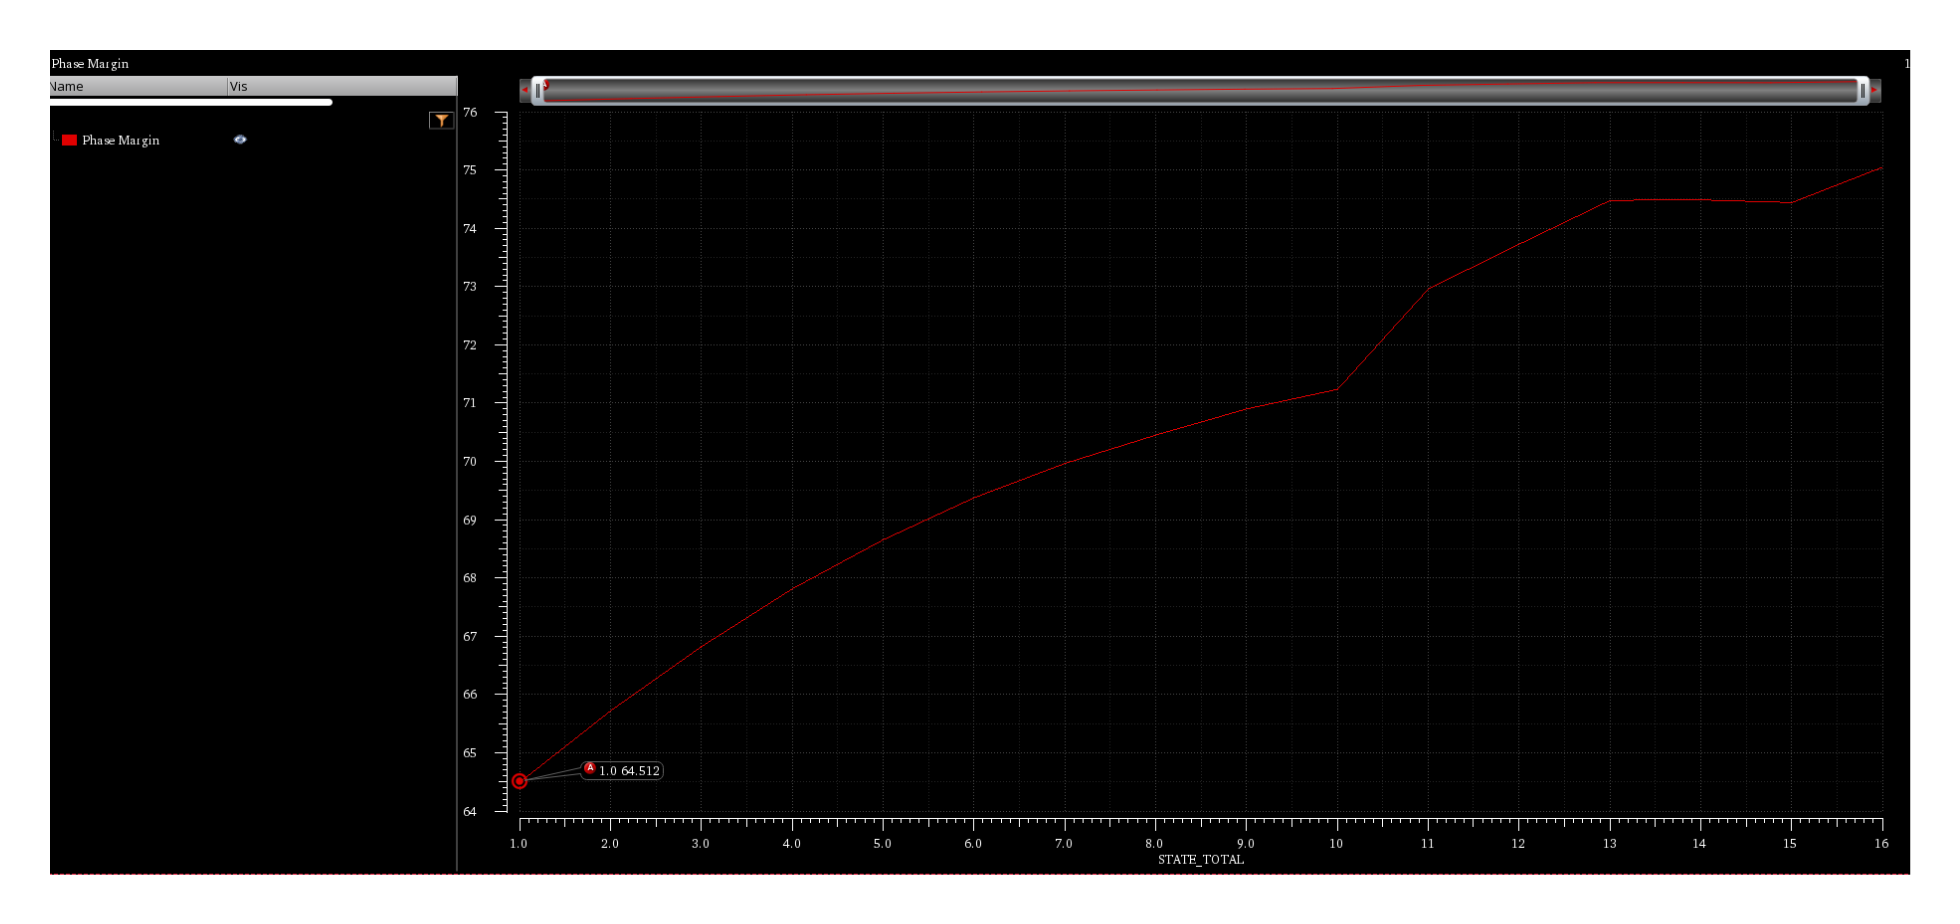
\includegraphics[width=1\linewidth]{images/Phase_margin_across_states.png}
  \caption{Phase Margin across states}
  \label{fig:Phase_margin_across_states.png}
\end{figure}

\begin{figure}[htbp]
  \centering
  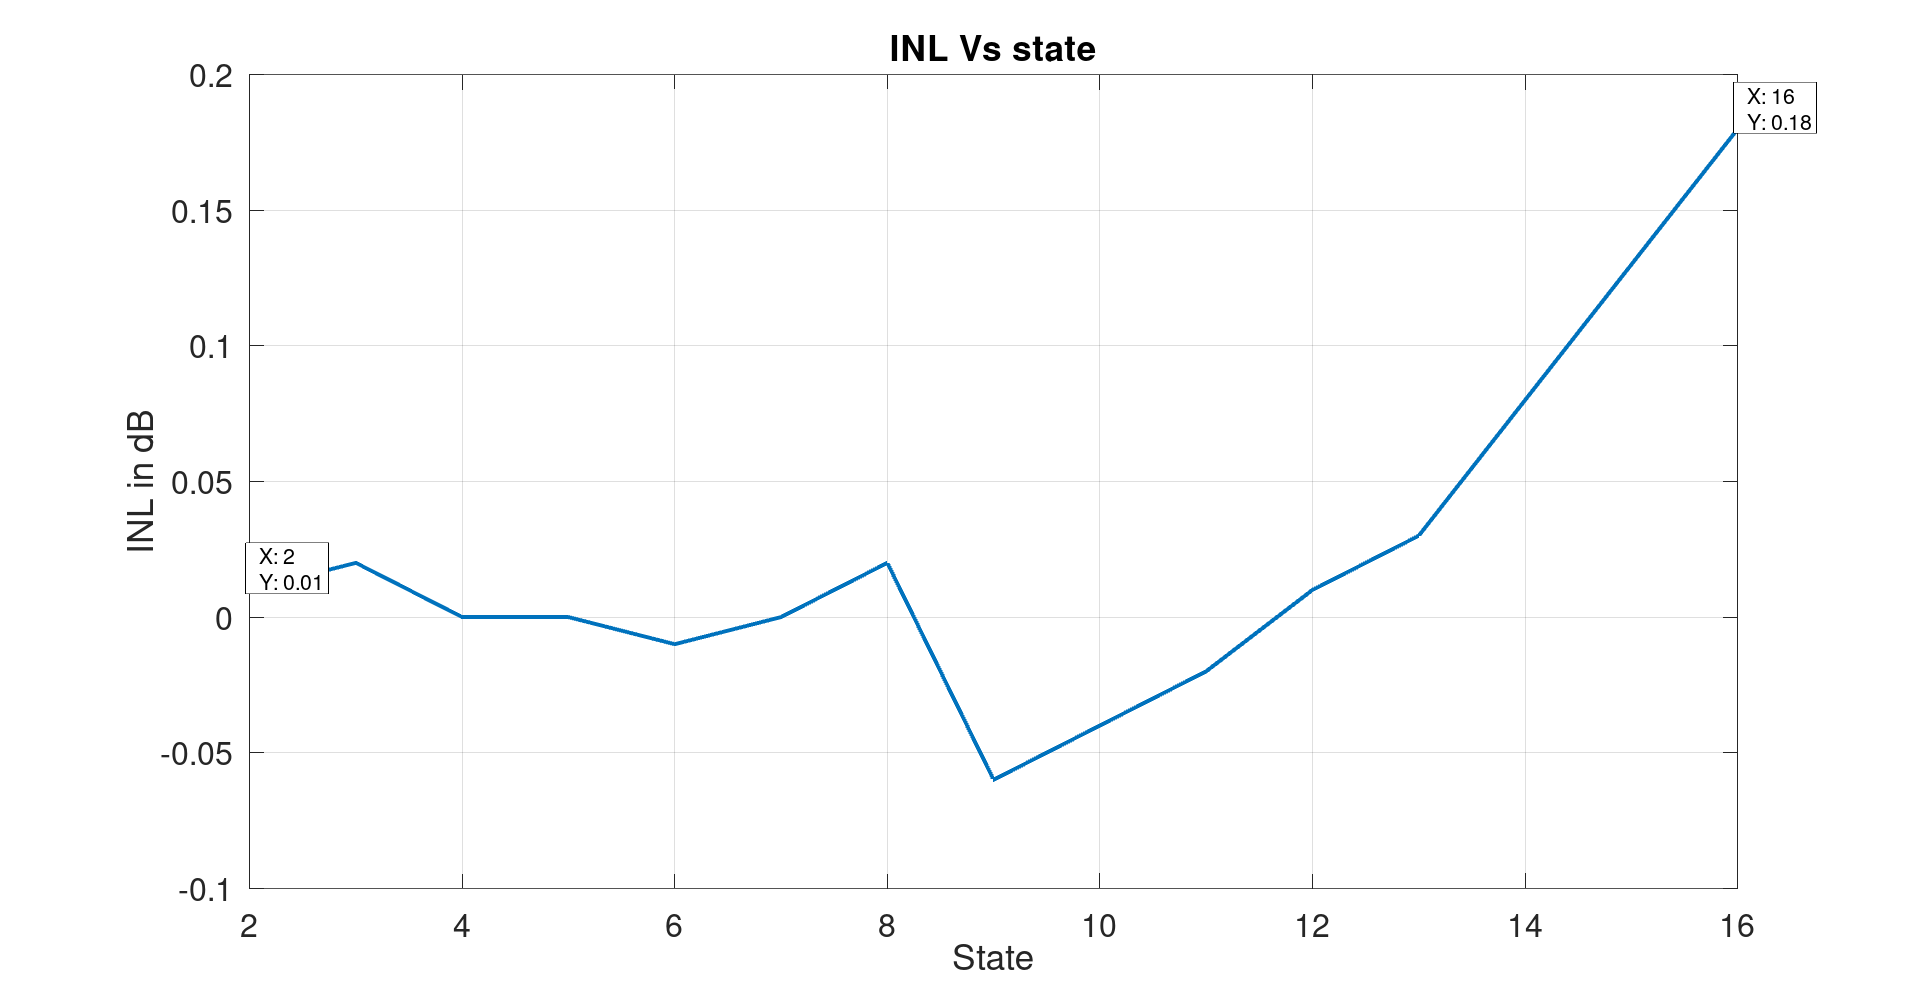
\includegraphics[width=1\linewidth]{images/INL_vs_state.png}
  \caption{INL Vs states}
  \label{fig:INL_vs_state.png}
\end{figure}
\begin{table}[htpb]
    \centering
    \caption{AC typical results summary}
    \label{tab:VGA_AC_results}
    \begin{tabular}{c|c}
        \textbf{Parameter} & \textbf{Value}  \\
         \toprule
        BW minimum & 625 MHz \\
        Max Gain & 39 dB \\
        NF (integrated up to 1.2GHz) & 2.7dB \\
        DNL max & 0.05dB \\
        INL max & 0.18dB \\
        PM min & 64 \\
    \end{tabular}
\end{table}
\clearpage

\subsection{HB simulation results}%
\label{sub:HB simulation results}
Two tone test with frequency 200MHz and 210MHz 
(worst case linearity) with 1mV amplitude, results are shown 
here in Figure~\ref{fig:OIP3_Vs_states_200MH.png} , this  variation
in OIP3 is due to gain variability since both LNA and resistive
feedback stage acts as Amplifier-Attenuator architecture (meaning)
constant IIP3 or more accurately Amplifier-Attenuator-Amplifier
Architecture, here is a comparison in 
Figure~\ref{fig:Dummy_Amp_att_arch_compared.png}

\begin{figure}[htbp]
  \centering
  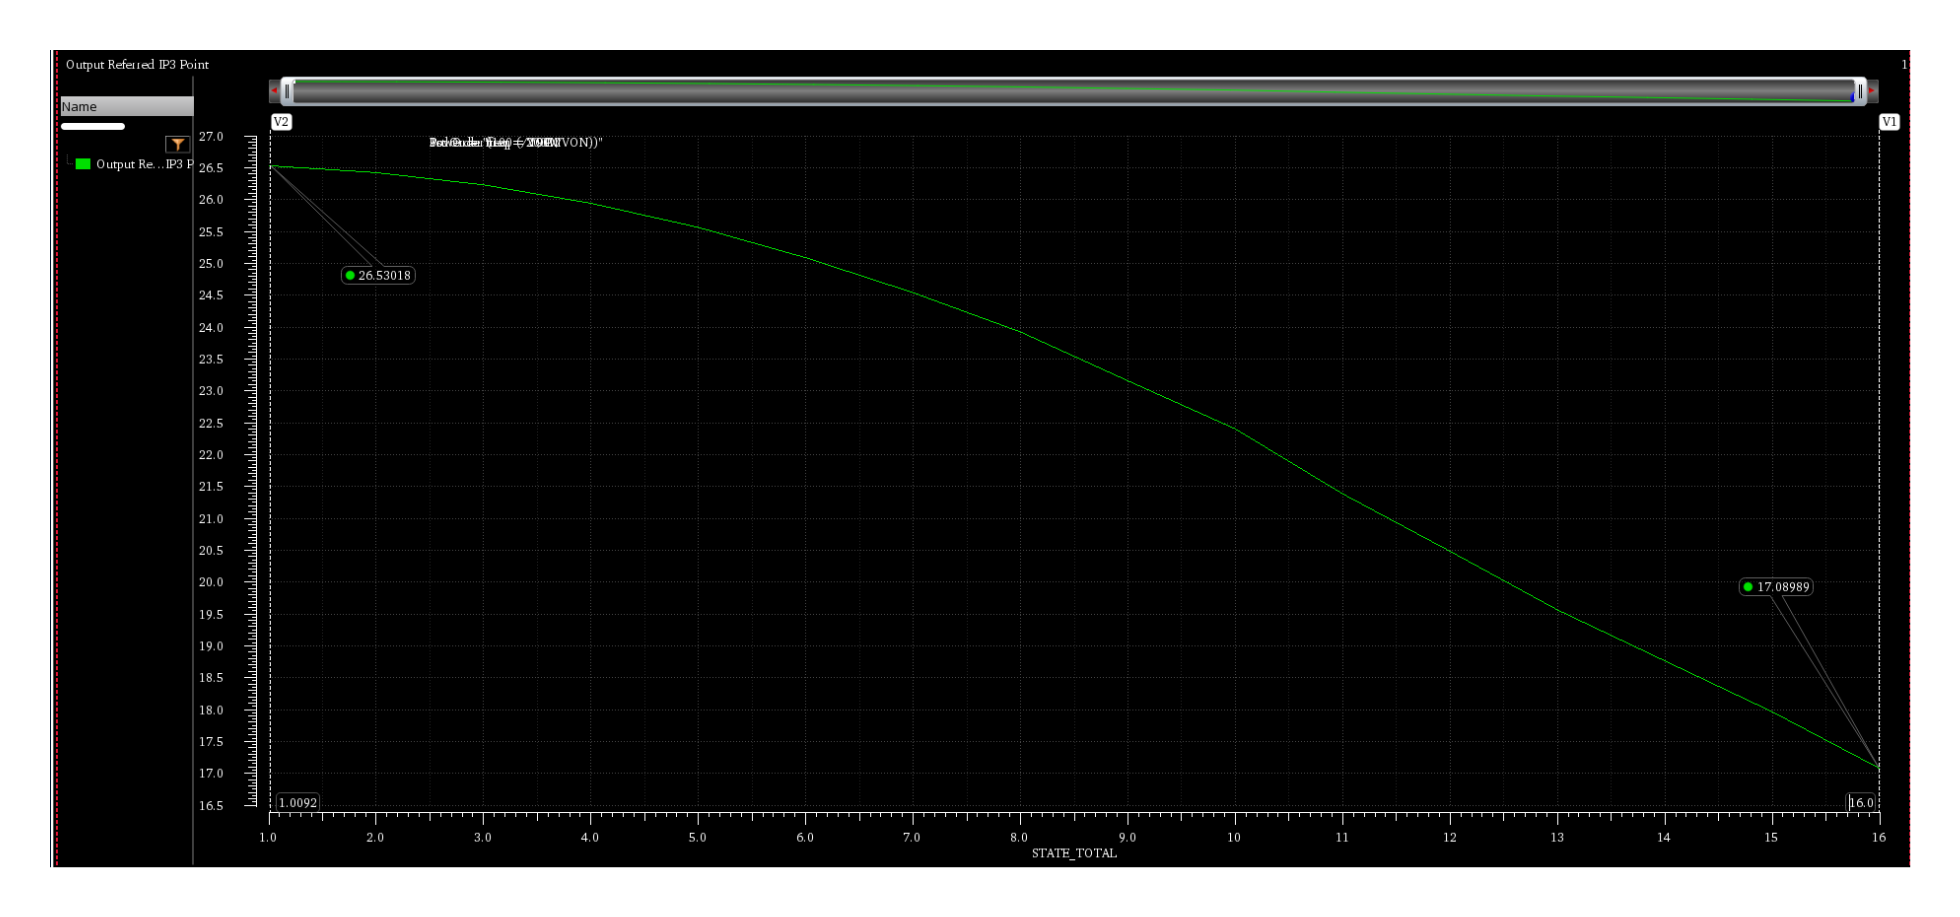
\includegraphics[width=1\linewidth]{images/OIP3_Vs_states_200MH.png}
  \caption{OIP3 Vs states at 200MHz}
  \label{fig:OIP3_Vs_states_200MH.png}
\end{figure}

\begin{figure}[!h]
  \centering
  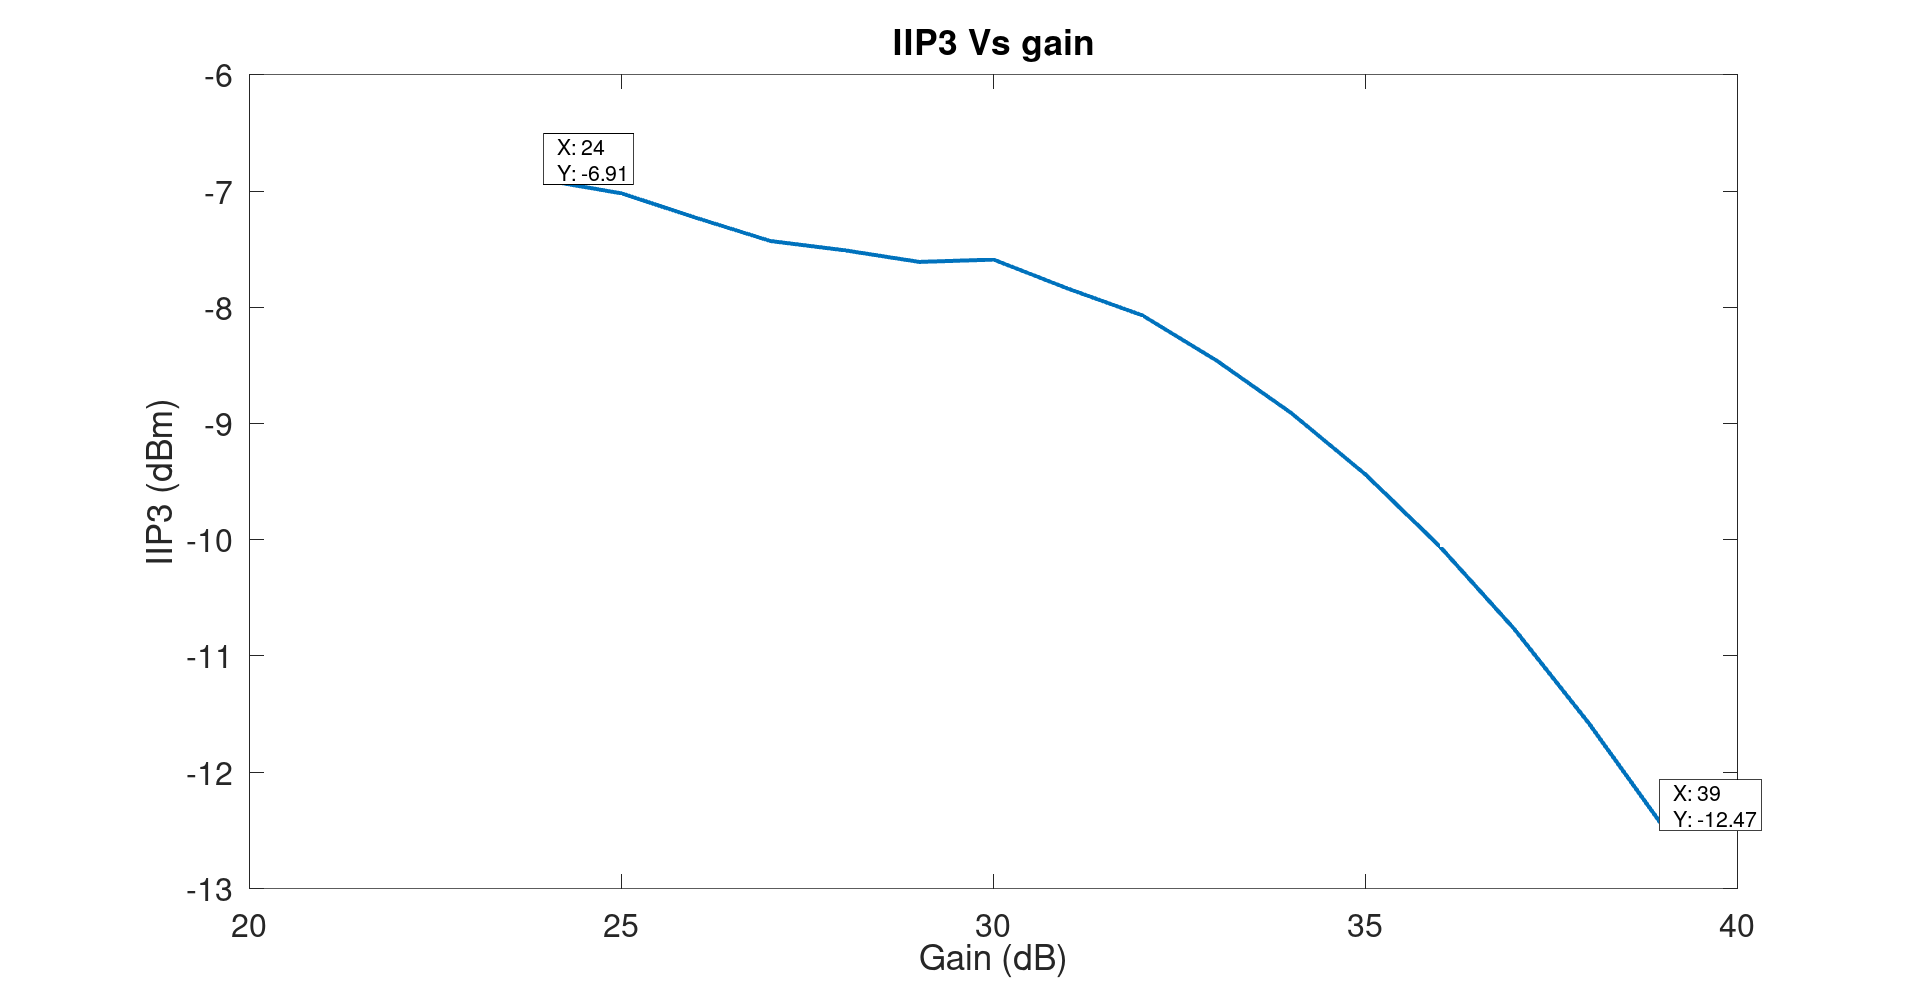
\includegraphics[width=1\linewidth]{images/IIP3_vs_Gain.png}
  \caption{IIP3 Vs gain}
  \label{fig:IIP3_vs_Gain.png}
\end{figure}
\begin{figure}[htbp]
  \centering
  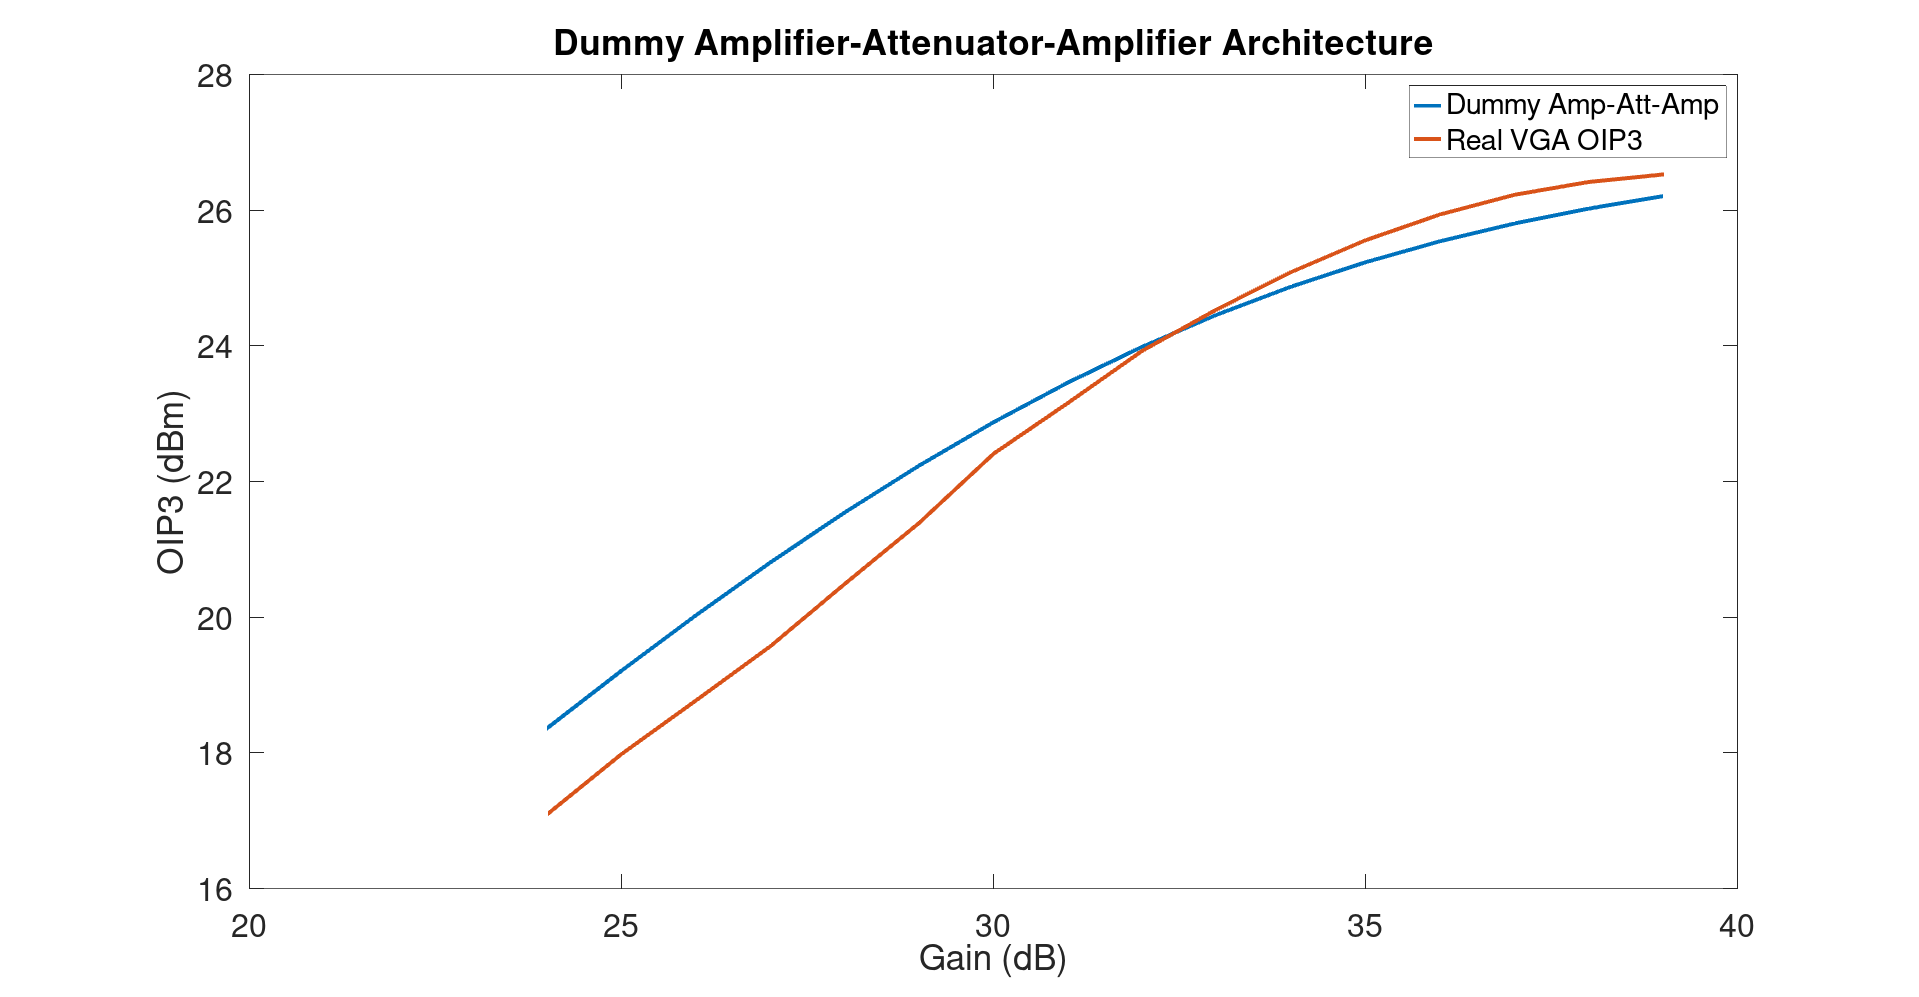
\includegraphics[width=1\linewidth]{images/Dummy_Amp_att_arch_compared.png}
  \caption{Dummy Amplifier-Attenuator-Amplifier Vs real OIP3}
  \label{fig:Dummy_Amp_att_arch_compared.png}
\end{figure}

\subsection{Corners}%
\label{sub:Corners}
Results are shown across corners, Bandwidth varies very much with
corners Figure~\ref{fig:BW_across_state.png} since Bandwidth 
depends on $g_m$ of the OPamp which varies across corners,
also OIP3 varies with corners (OIP3 depends on Bandwidth)
Figure~\ref{fig:OIP3_Vs_states_across_corners.png} , on the
other hand DNL and INL are doesn't vary very much with corners
Figure~\ref{fig:DNL_across_corner.png} and
Figure~\ref{fig:INL_across_corners.png}, Noise figure at 
max gain (Not shown) NF = 3.43 for slow hot corner and 2.13 for
fast cold corner.

\begin{figure}[htbp]
  \centering
  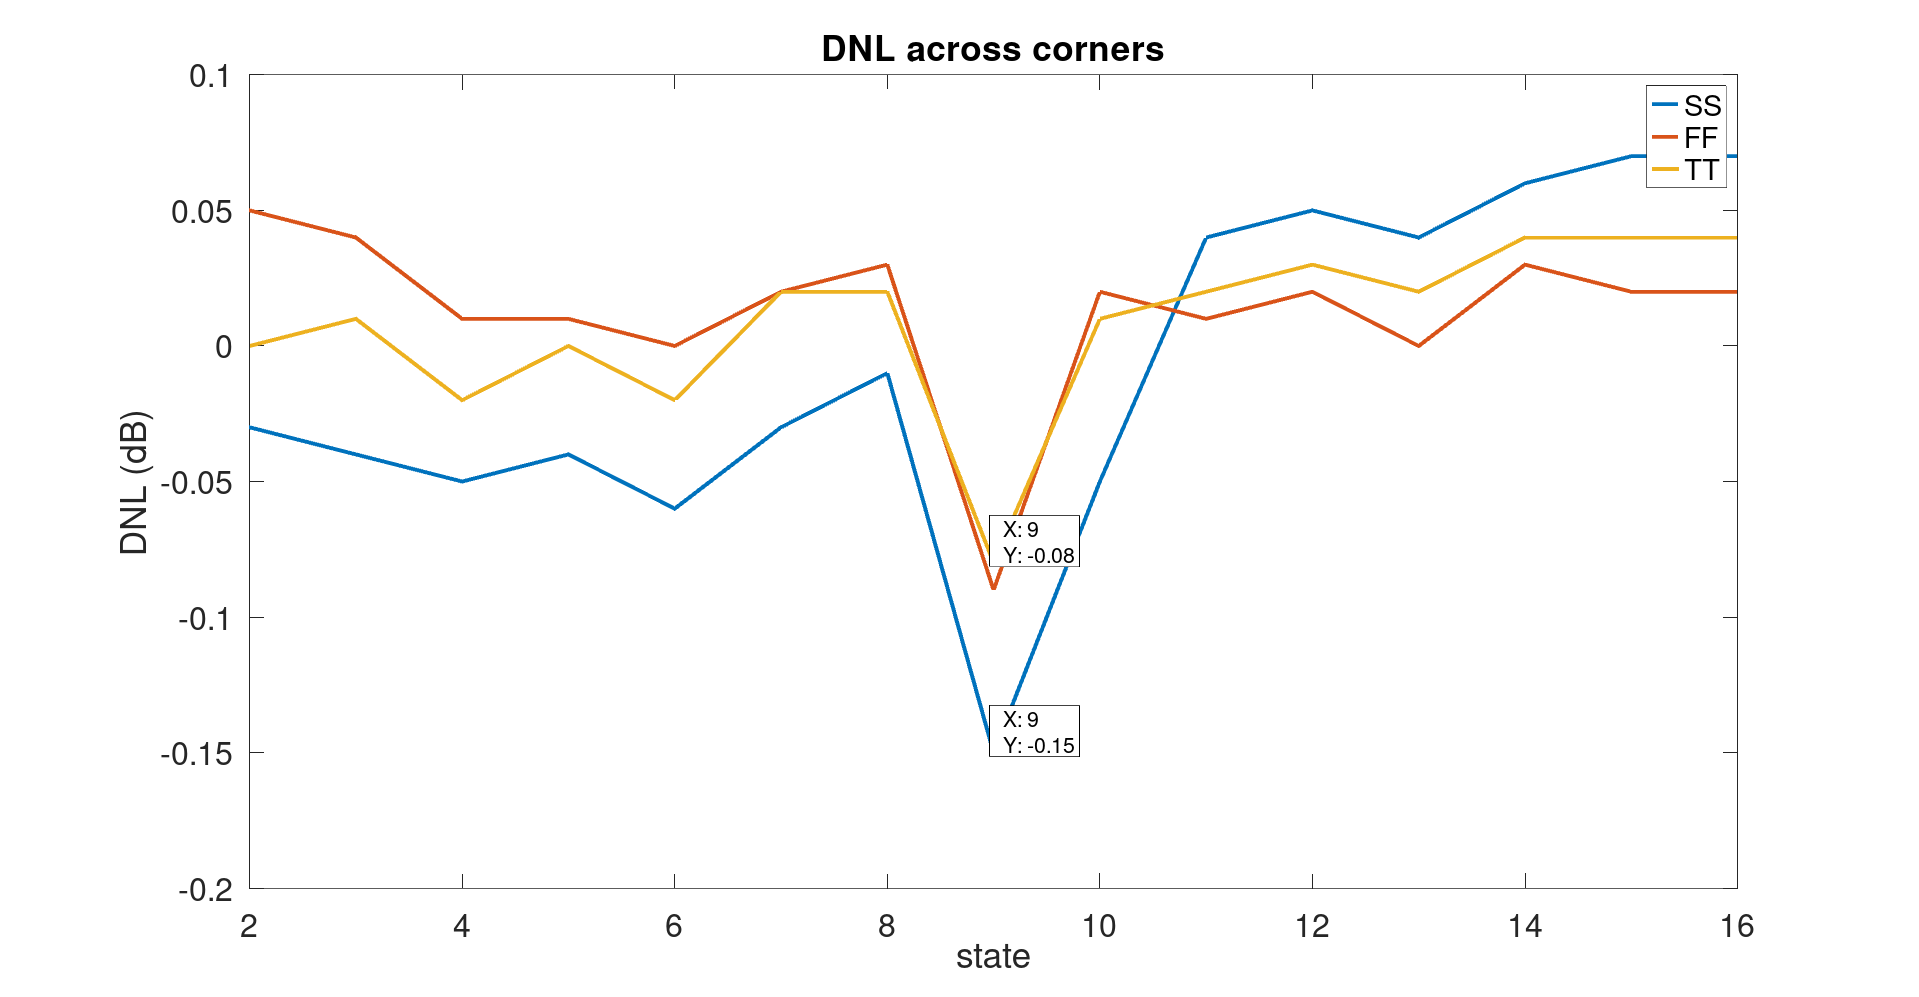
\includegraphics[width=1\linewidth]{images/DNL_across_corner.png}
  \caption{DNL Vs states across corners}
  \label{fig:DNL_across_corner.png}
\end{figure}

\begin{figure}[htbp]
  \centering
  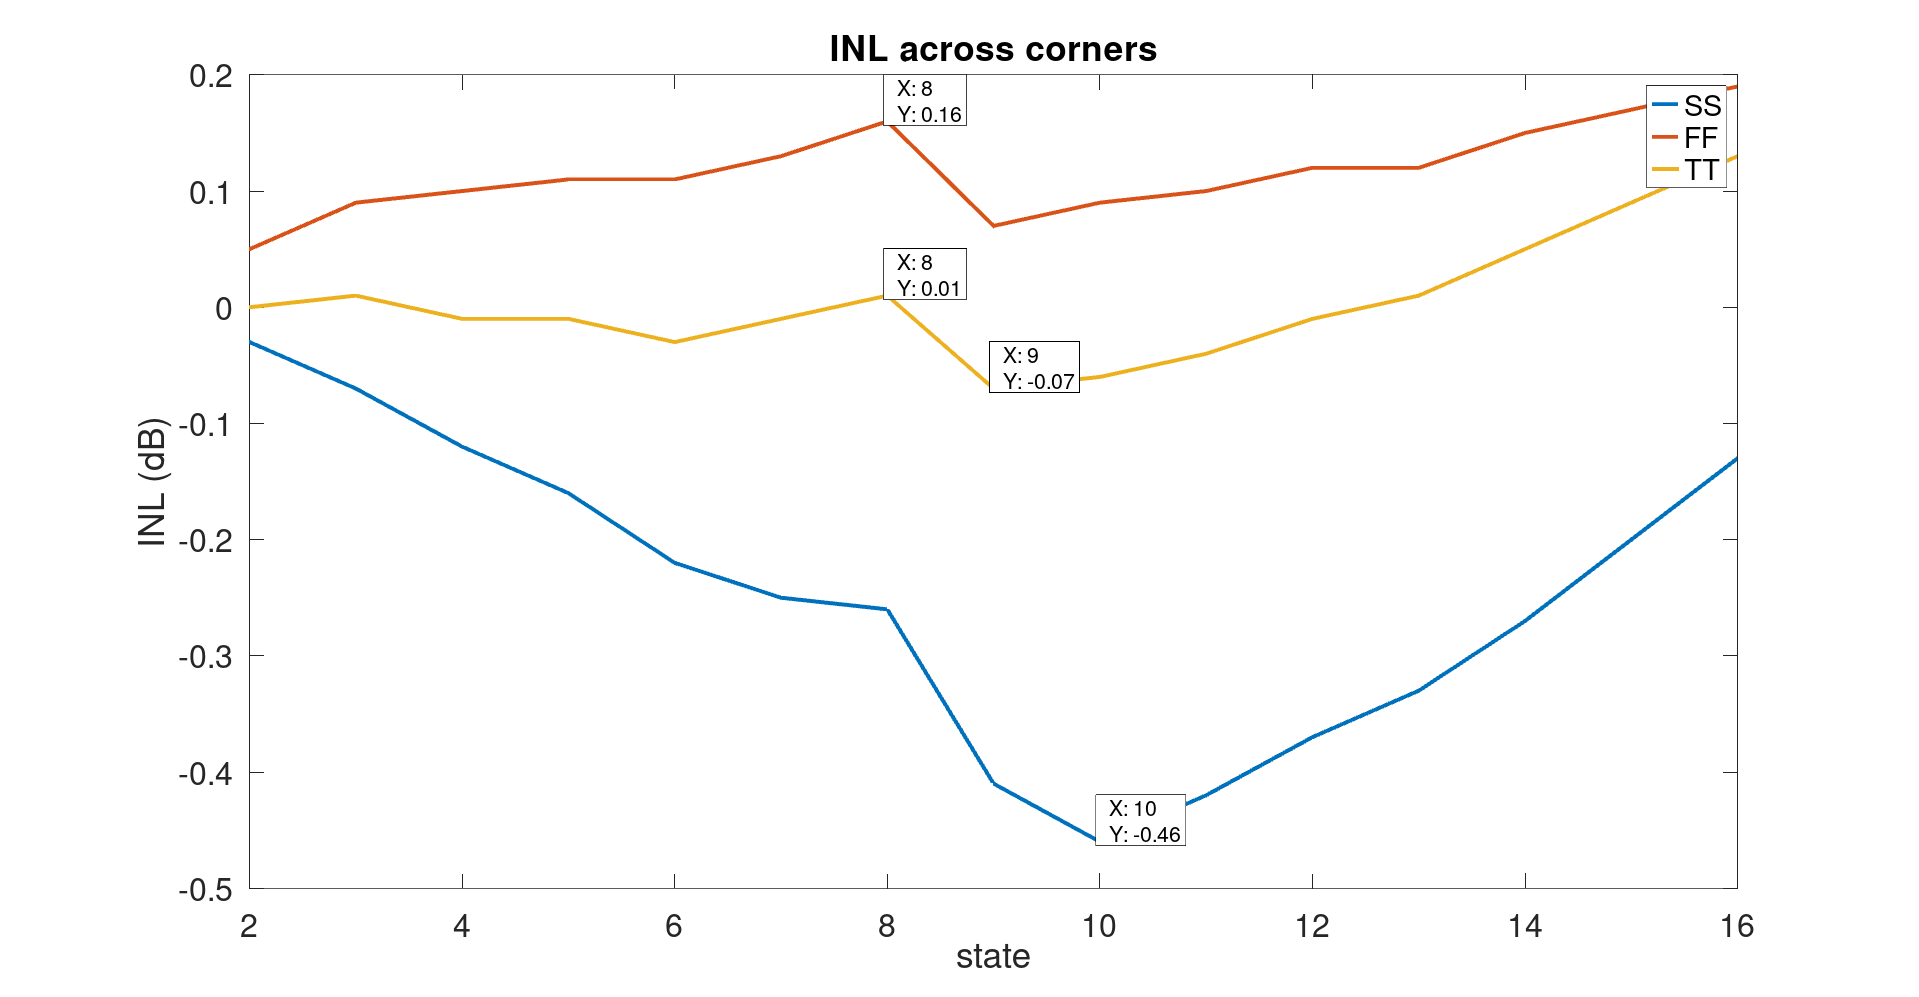
\includegraphics[width=1\linewidth]{images/INL_across_corners.png}
  \caption{INL Vs states across corners}
  \label{fig:INL_across_corners.png}
\end{figure}

\begin{figure}[htbp]
  \centering
  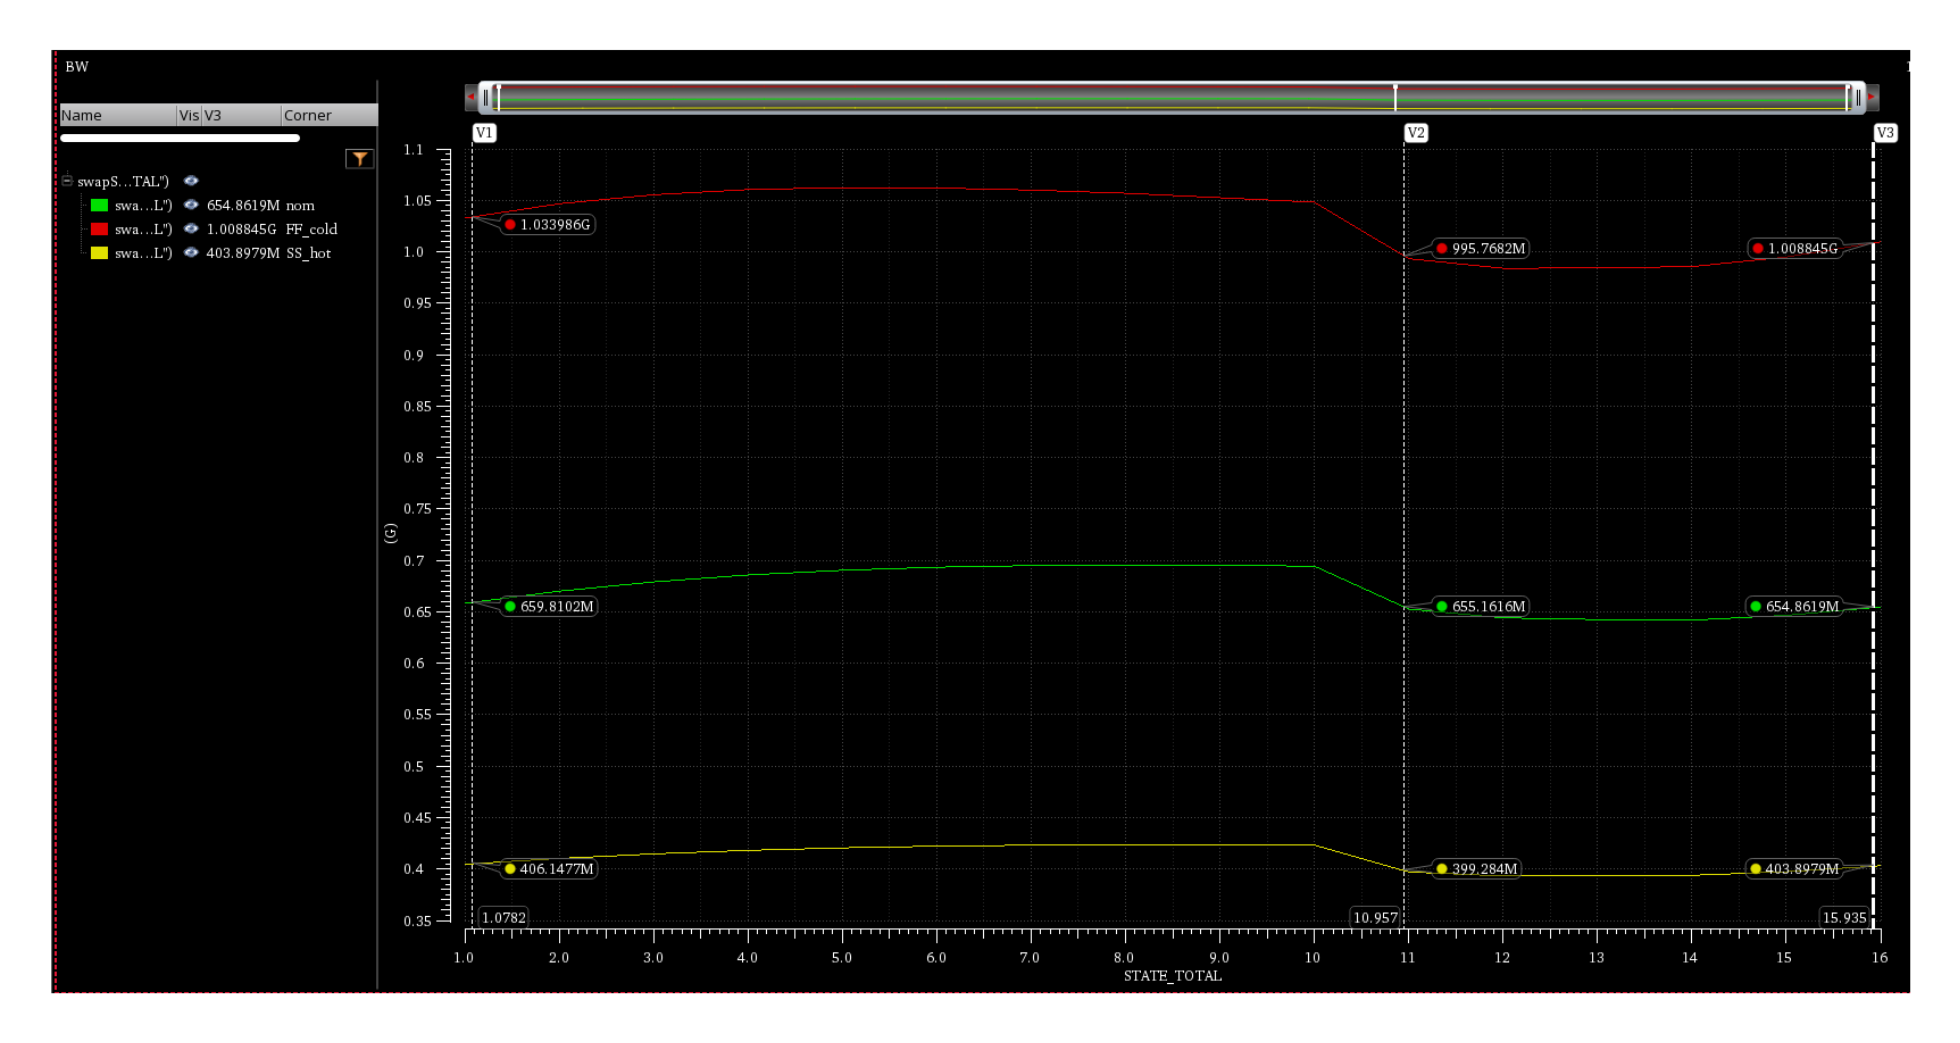
\includegraphics[width=1\linewidth]{images/VGA_BW_across_corners.png}
  \caption{BW Vs states across corners}
  \label{fig:VGA_BW_across_corners.png}
\end{figure}

\begin{figure}[htbp]
  \centering
  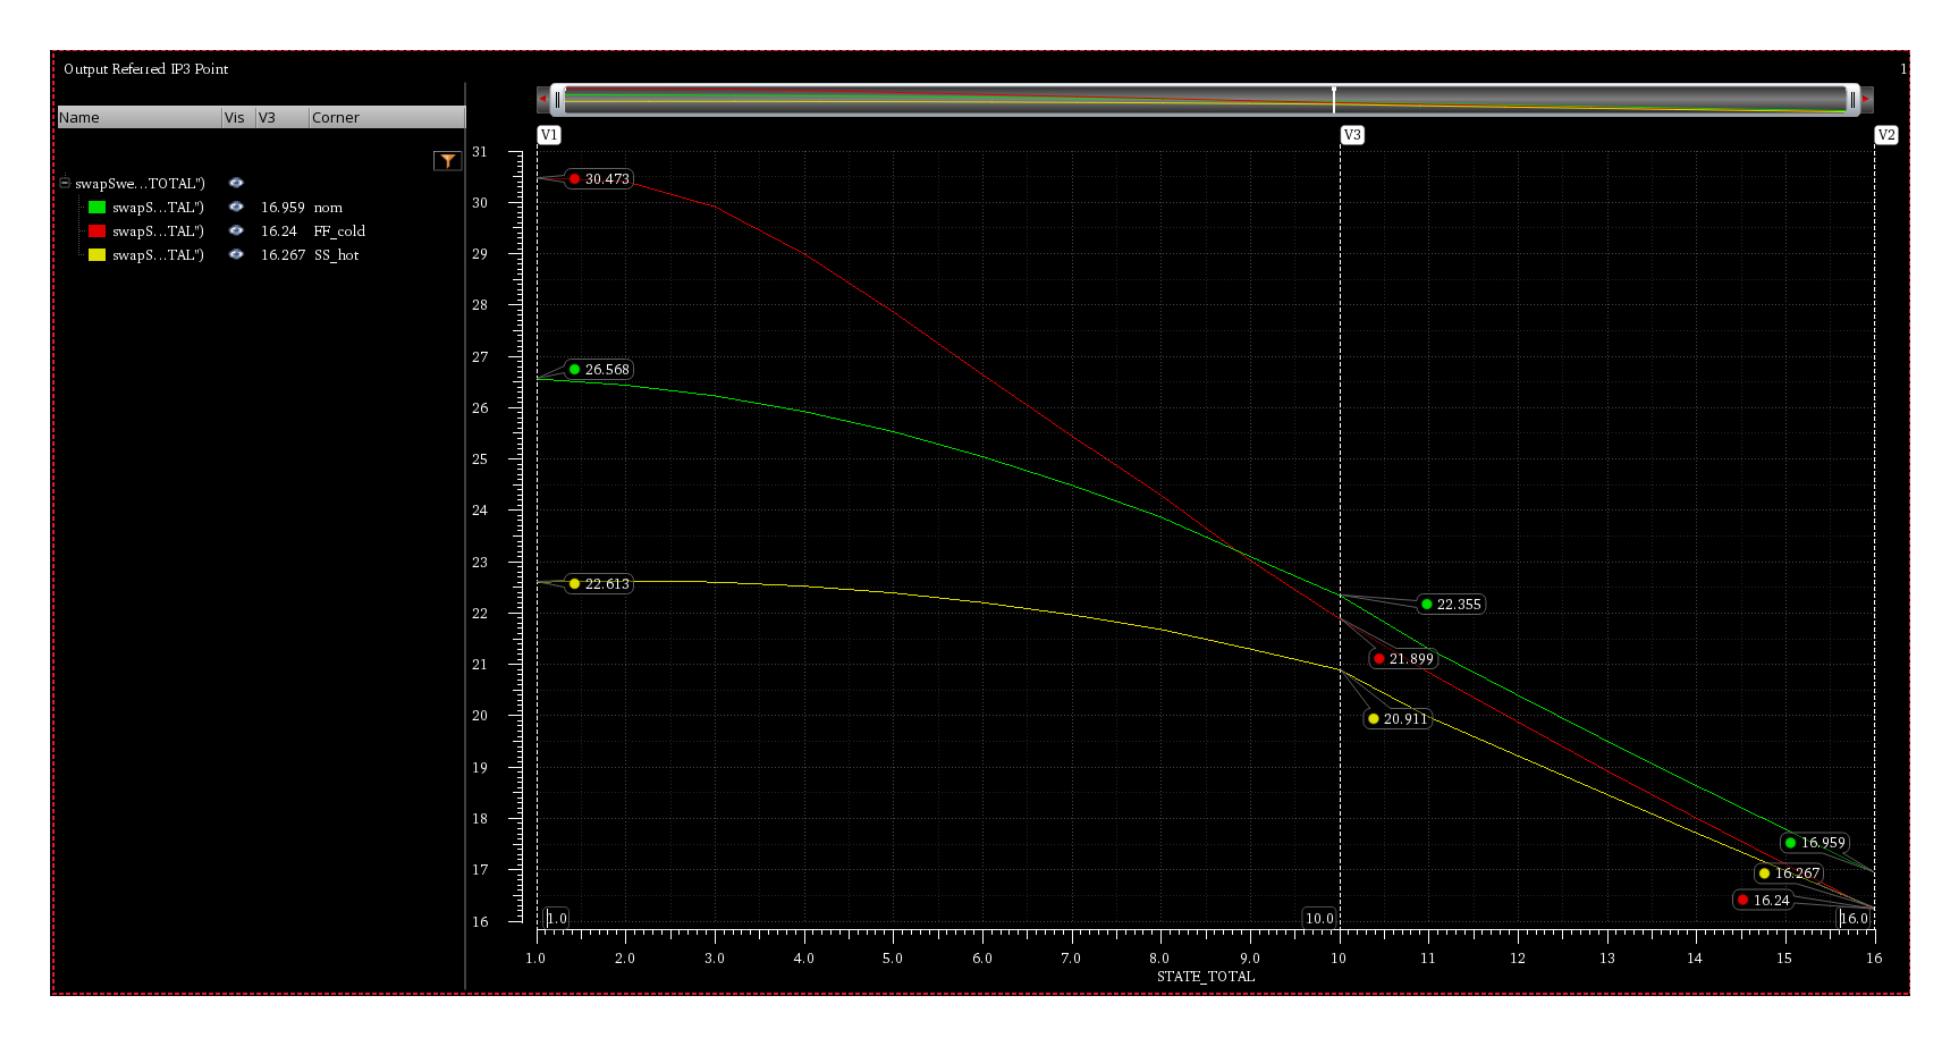
\includegraphics[width=1\linewidth]{images/OIP3_Vs_states_across_corners.png}
  \caption{OIP3 Vs states across corners}
  \label{fig:OIP3_Vs_states_across_corners.png}
\end{figure}

\begin{figure}[htbp]
  \centering
  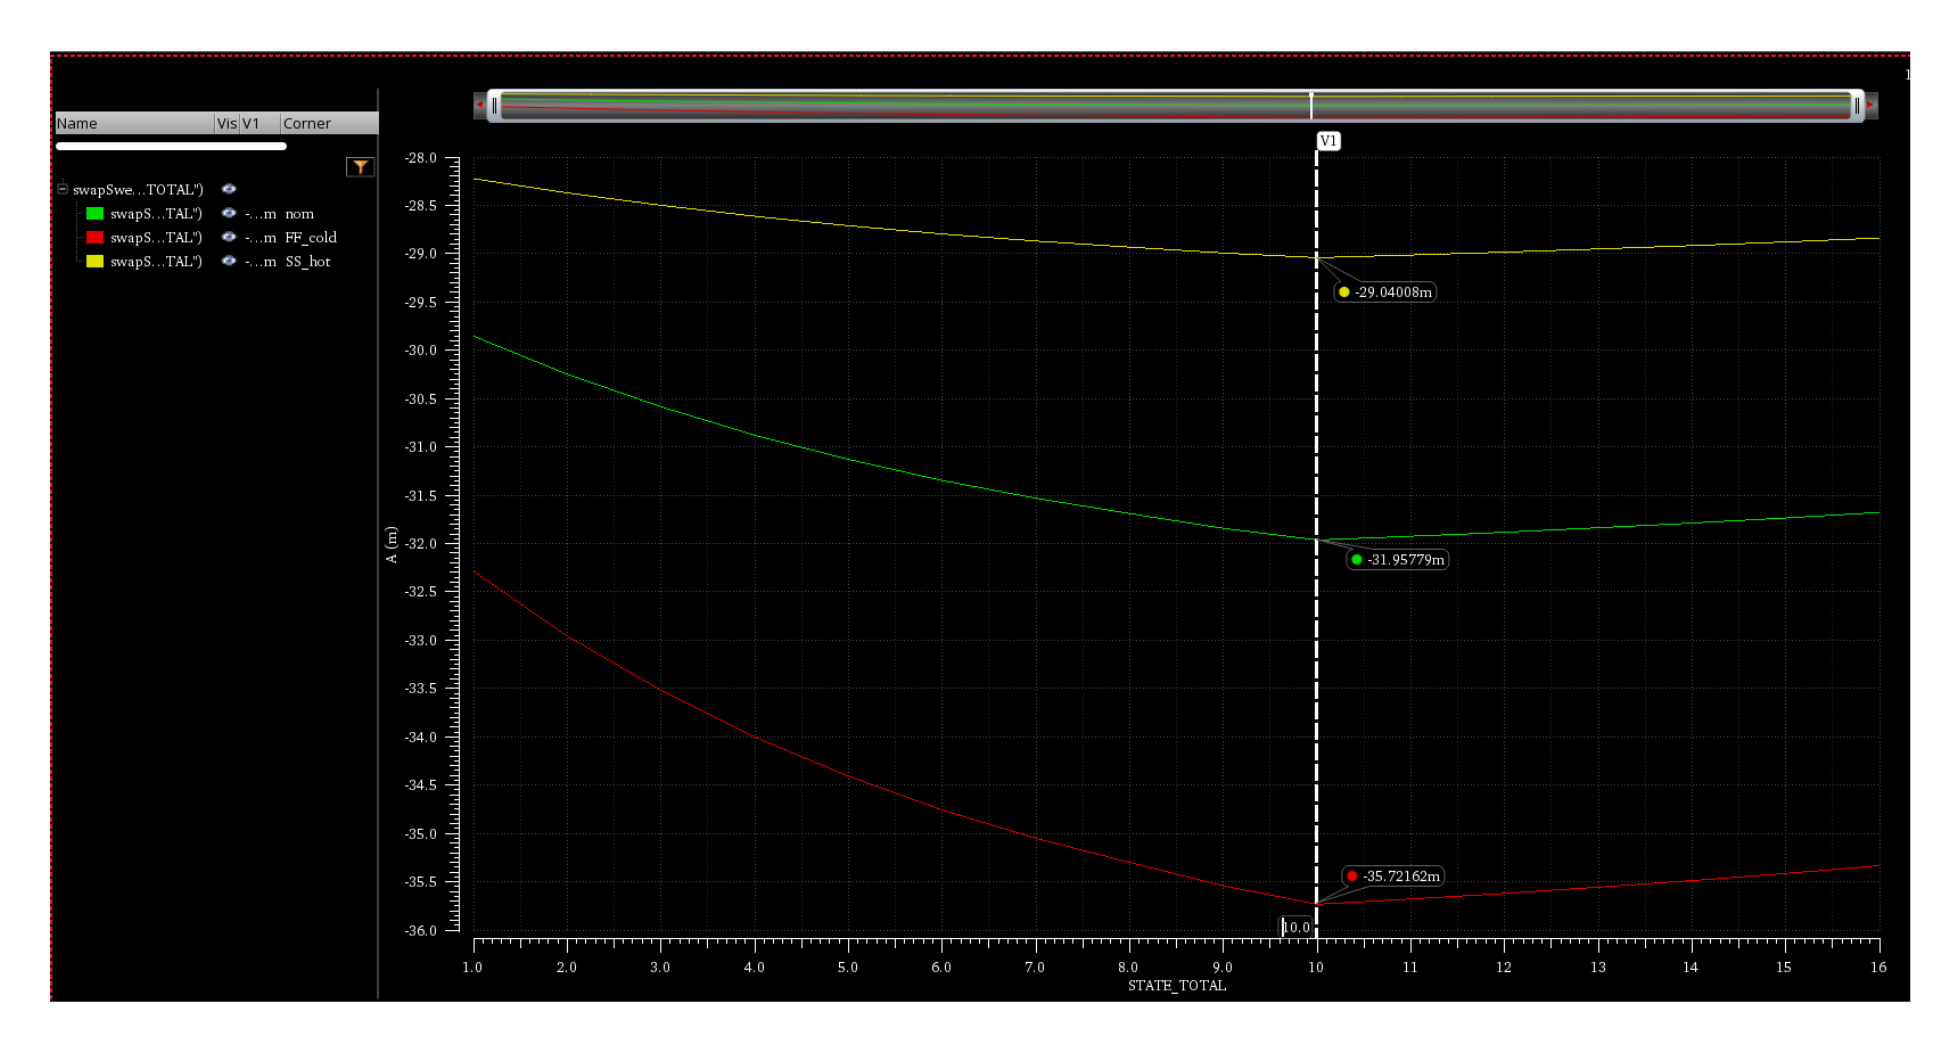
\includegraphics[width=1\linewidth]{images/DC_current_Vs_states_across_corners.png}
  \caption{DC current Vs states across corners}
  \label{fig:DC_current_Vs_states_across_corners.png}
\end{figure}
\clearpage

\section{Summary}%
The final VGA acts as Amplifier-Attenuator-Amplifier architecture,
which explains why linearity degrades with the states , here
is the achieved specifications
\begin{table}[htpb]
    \centering
    \caption{Achieved Specifications}
    \label{tab:VGA_achieved_specs}

    \begin{tabular}{l c c c c}
        \textbf{Parameter} & \textbf{Specification}  &
        \textbf{Fast Cold corner}&\textbf{Typical}  &\textbf{Slow
        Hot corner} \\
        \toprule
            Supply & & 1.68 & 1.6 & 1.52 \\
            Temperature & & -25 & 27 & 125 \\
            BW & 600MHz & 995MHz & 625MHz & 399MHz \\
            Max Gain & 39 dB & 39 dB  & 39 dB & 39 dB \\
            Gain Range & 15 dB & 15 dB &15dB & 15dB \\
            NF (at Max gain) & 3 dB & 2.13 dB & 2.7 dB & 3.43 dB \\
            IIP3 (at min gain) & 1 dBm & -7.76 dBm & -7 dBm & -7.7dBm \\
            Power Consumption & & 57.1 mW & 51 mW & 46.4 mW \\ 
            \bottomrule
    \end{tabular}
\end{table}
